\documentclass{article}
\usepackage[brazil]{babel}
\usepackage[utf8]{inputenc}
\usepackage{url}
\usepackage{multicol}
\usepackage[bottom=2cm,top=2cm,left=2cm,right=2cm]{geometry}
\usepackage{graphicx}
\usepackage{float}
\usepackage{caption}
\usepackage[dvipsnames]{xcolor}
\usepackage{tikz}
\usepackage{amssymb}
\usepackage{setspace}
\usepackage{indentfirst}
\usepackage{mathtools}
\usepackage{amsmath}
\usepackage{subfigure}

\title{Lista 2\\
\large Sistemas Baseados em Conhecimento: \texttt{[MAC0444]}}
\author{Julia Leite - \texttt{11221797}}

\begin{document}

    \maketitle

    \textbf{Ex 1}

    \begin{itemize}
        \item [-] vaiBem(Maria)
        \item [-] fezEx(João)
        \item [-] $\forall$x (fezEx(x) $\rightarrow$ vaiBem(x))
        \item [-] $\forall$y (vaiBem(y) $\rightarrow$ mediaAlta(y))
        \item [-] $\forall$z (mediaAlta(z) $\rightarrow$ aprovado(z, mac444))
    \end{itemize}

    Nosso KB:

    \begin{itemize}
        \item [-] vaiBem(Maria)
        \item [-] fezEx(João)
        \item [-] $\neg$ fezEx(x) $\lor$ vaiBem(x)
        \item [-] $\neg$ vaiBem(y) $\lor$ mediaAlta(y)
        \item [-] $\neg$ mediaAlta(z) $\lor$ aprovado(z, mac 444)
    \end{itemize}

    Primeiro vamos mostrar que Maria foi aprovada em mac 444, mostrando que 
    $KB \vDash \neg aprovado(Maria, mac 444)$ é Falso

    \begin{figure}[H]
        \centering
        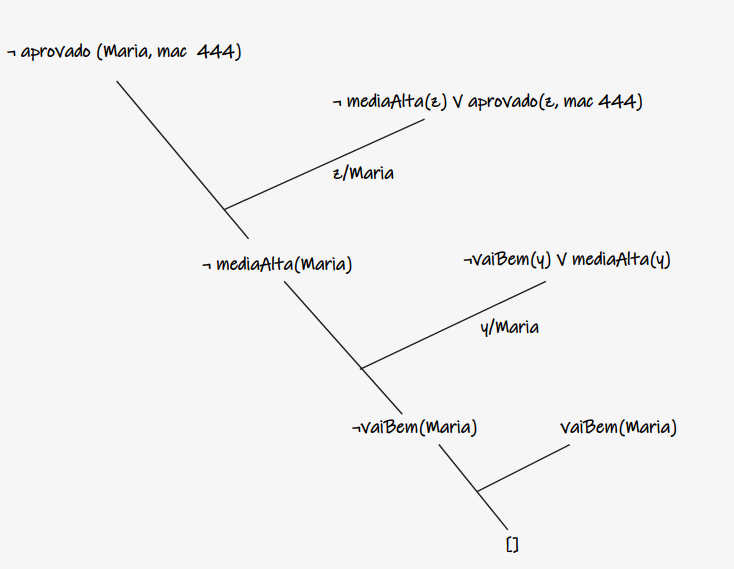
\includegraphics[width=12cm]{img/maria.png}
    \end{figure}
    
    Agora, analogamente, vamos provar que João foi aprovado em mac 444

    \begin{figure}[H]
        \centering
        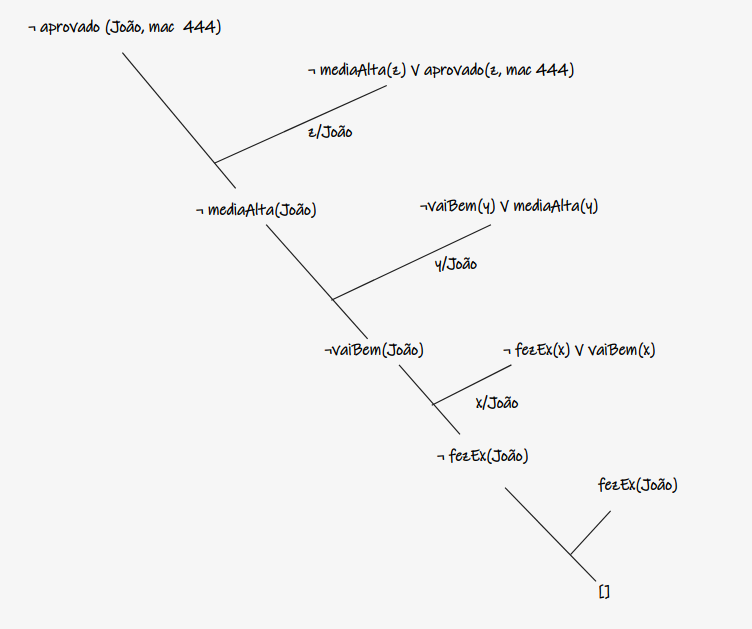
\includegraphics[width=12cm]{img/joao.png}
    \end{figure}

    \textbf{Ex 2}

    \begin{itemize}
        \item [-] $[\neg A_1(x), \neg A_2(x), P(x)]$
        \item [-] $[\neg B_1(x), \neg B_2(x), A_1(x)]]$
        \item [-] $[\neg B_3(x), \neg B_4(x), A_2(x)]$
        \item [-] [$B_1$(a)]
        \item [-] [$B_2$(a)]
        \item [-] [$B_3$(a)]
        \item [-] [$B_4$(a)]
    \end{itemize}

Vamos mostrar que o backward chaining responde SIM
com objetivo P(a)\\

    \texttt{[P(a)]}\\
    \texttt{[$A_1$(a), $A_2$(a)]}\\
    \texttt{[$B_1$(a), $B_2$(a), $A_2$(a)]}\\
    \texttt{[$B_2$(a), $A_2$(a)]}\\
    \texttt{[$A_2$(a)]}\\
    \texttt{[$B_3$(a), $B_4$(a)]}\\
    \texttt{[$B_4$(a)]}\\
    \texttt{[]}\\

    \newpage

    \textbf{Ex 3}

    Programa:\\
    \texttt{result([ \_ , E | L ] , [ E | M ]) : - ! , result(L , M ).\\
    result(\_ , []).}\\

    Consulta:\\
    \texttt{result ([ a , b , c , d , e , f , g ] , X ).}\\

    \textbf{a)} A resposta do prolog para a consulta seria:

    \texttt{X = [b, d, f]}\\

    \textbf{b)} 

    Esse programa recebe uma lista e armazena na variável passada como parâmetro (\texttt{X}) outra lista, 
    apenas com os elementos de índice par da primeira (ou seja, o 2º elemento,
    4º, ...), utilizando recursão.

    A cada execução de \texttt{result} armazenamos o 2º elemento da lista recebida, e chamamos
    recursivamente para o restante da lista, como o 1º elemento não é 
    utilizado, uma variável anônima é empregada para representá-lo.

    Primeiro verificamos se conseguimos decompor a lista recebida como
    descrito acima (E, L e M),
    caso contrário, retornamos uma lista vazia (base da recursão).

    A presença do corte, então, garante que apenas a solução com todos
    os elementos de índice par seja retornada, já que impede o retrocesso
    do Prolog no ponto de escolha anterior. Sem esse recurso, outras soluções também
    seriam consideradas, como apenas o 2º elemento, apenas a lista vazia, entre outras.\\


    \textbf{Ex 4}

    \textbf{a)} Regra para o predicado: \texttt{avof(Mul,Pess)} em que \texttt{Mul} seja avó de \texttt{Pess}

    \begin{figure}[H]
        \centering
        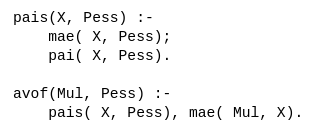
\includegraphics[width=6cm]{img/4a.png}
    \end{figure}

    \textbf{c)} Regra para o predicado: \texttt{bisavom(Hom,Pess}) que é verdadeiro se \texttt{Hom} for bisavô de \texttt{Pess}.

    \begin{figure}[H]
        \centering
        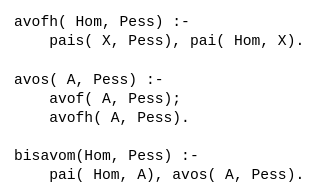
\includegraphics[width=6cm]{img/4c.png}
    \end{figure}

    \textbf{d)} Regra para o predicado: \texttt{primo\_1(P1, P2)} que é verdadeiro se \texttt{P1} e \texttt{P2} forem primos em primeiro grau.

    \begin{figure}[H]
        \centering
        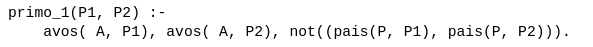
\includegraphics[width=10cm]{img/4d.png}
    \end{figure}

    \textbf{f)} Regra para o predicado: \texttt{maior\_de\_idade(Pess)} que é verdadeiro se \texttt{Pess} for maior de idade.

    \begin{figure}[H]
        \centering
        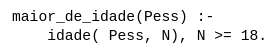
\includegraphics[width=6cm]{img/4f.png}
    \end{figure}

    \newpage

    \textbf{g)} Regra para o predicado: \texttt{pessoas(Lista)} que devolve a \texttt{Lista} de todas as pessoas existentes na base de conhecimento

    \begin{figure}[H]
        \centering
        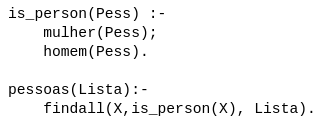
\includegraphics[width=6cm]{img/4g.png}
    \end{figure}

    \textbf{h)} Regra para o predicado: \texttt{mais\_velho(Pess)} que retorna a pessoa mais velha que consta na base de conhecimento.

    \begin{figure}[H]
        \centering
        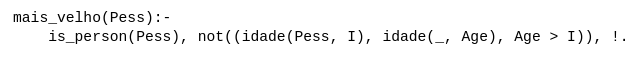
\includegraphics[width=12cm]{img/4h.png}
    \end{figure}

    \textbf{i)} Regra para o predicado: \texttt{lista\_pessoas(Lista, Sexo)} que retorna uma \texttt{Lista} de todas as pessoas do \texttt{Sexo}
    indicado \texttt{(m/f)}, incluindo as suas respectivas idades

    \begin{figure}[H]
        \centering
        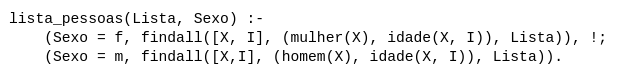
\includegraphics[width=12cm]{img/4i.png}
    \end{figure}

    \textbf{j)} Regra para o predicado: \texttt{adequados(Hom, Mul)} que é verdadeiro se \texttt{Hom} for um homem, \texttt{Mul} for uma mulher e o
    homem for (no máximo) 2 anos mais novo do que a mulher ou 10 anos mais velho do que
    ela e se ambos não tiverem nenhuma relação de parentesco nem nenhum deles for casado.

    \begin{figure}[H]
        \centering
        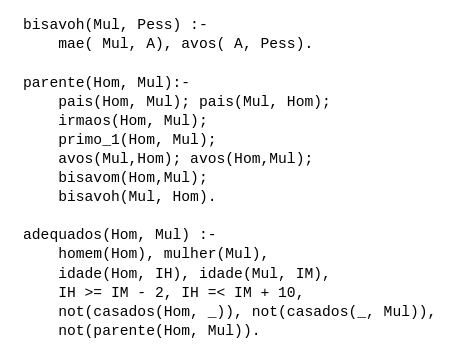
\includegraphics[width=10cm]{img/4j.png}
    \end{figure}

    Obs: consideramos parentes pais, irmãos, avó ou avô, bisavô e 
    bisavó e primos de primeiro grau.

\end{document}
